\let\negmedspace\undefined
\let\negthickspace\undefined
\documentclass[journal]{IEEEtran}
\usepackage[a5paper, margin=10mm, onecolumn]{geometry}
\usepackage{lmodern} % Ensure lmodern is loaded for pdflatex
\usepackage{tfrupee} % Include tfrupee package

\setlength{\headheight}{1cm} % Set the height of the header box
\setlength{\headsep}{0mm}     % Set the distance between the header box and the top of the text

\usepackage{gvv-book}
\usepackage{gvv}
\usepackage{cite}
\usepackage{amsmath,amssymb,amsfonts,amsthm}
\usepackage{algorithmic}
\usepackage{graphicx}
\graphicspath{{./figs/}}
\usepackage{textcomp}
\usepackage{xcolor}
\usepackage{txfonts}
\usepackage{listings}
\usepackage{enumitem}
\usepackage{mathtools}
\usepackage{gensymb}
\usepackage{comment}
\usepackage[breaklinks=true]{hyperref}
\usepackage{tkz-euclide} 
\usepackage{listings}
\usepackage{gvv}                                        
\def\inputGnumericTable{}                                 
\usepackage[latin1]{inputenc}                                
\usepackage{color}                                            
\usepackage{array}                                            
\usepackage{longtable}                                       
\usepackage{calc}                                             
\usepackage{multirow}                                         
\usepackage{hhline}                                           
\usepackage{ifthen}                                           
\usepackage{lscape}
\usepackage{circuitikz}
\tikzstyle{block} = [rectangle, draw, fill=blue!20, 
text width=4em, text centered, rounded corners, minimum height=3em]
\tikzstyle{sum} = [draw, fill=blue!10, circle, minimum size=1cm, node distance=1.5cm]
\tikzstyle{input} = [coordinate]
\tikzstyle{output} = [coordinate]
\begin{document}
\bibliographystyle{IEEEtran}
\vspace{3cm}
\title{2.5.4}
\author{EE25BTECH11050-Hema Havil}
\maketitle
	% \newpage
	% \bigskip
	{\let\newpage\relax\maketitle}
	
	\renewcommand{\thefigure}{\theenumi}
	\renewcommand{\thetable}{\theenumi}
	\setlength{\intextsep}{12pt} % Space between text and floats
	
	\numberwithin{equation}{enumi}
	\numberwithin{figure}{enumi}
	\renewcommand{\thetable}{\theenumi}
	
	\textbf{Question}:\\
    
         If $\vec{a}=2\hat{i}+y\hat{j}+\hat{k}$ and $\vec{b}=\hat{i}+2\hat{j}+3\hat{k}$ are two vectors for which the vector ($\vec{a}+\vec{b}$) is perpendicular to the vector ($\vec{a}-\vec{b}$), then find all the possible values of y.\\
         
         \solution \\
         Let the given vectors be :\\ 
         \begin{align}
             \vec{a}=\myvec{2\\y\\1}  \vec{b}=\myvec{1\\2\\3}
         \end{align}
         Given that $\vec{a}+\vec{b}$ and $\vec{a}-\vec{b}$  are perpendicular, then \\
         \begin{align}
             \brak{\vec{a}+\vec{b}}^T\brak{\vec{a}-\vec{b}}=0
         \end{align}
         \begin{align}
             \vec{a}^T\vec{a}-\vec{b}^T\vec{b}=0
         \end{align}
         \begin{align}
             \vec{a}^T\vec{a}=\vec{b}^T\vec{b}
         \end{align}
         The values of $\vec{a}^T\vec{a}$ and $\vec{b}^T\vec{b}$ can be calculated by,
         \begin{align}
             \vec{a}^T\vec{a}=\myvec{2\;y\;1}\myvec{2\\y\\1}=4+y^2+1=5+y^2
         \end{align}
         \begin{align}
             \vec{b}^T\vec{b}=\myvec{1\;2\;3}\myvec{1\\2\\3}=1+4+9=14
         \end{align}
         From equation 0.4,\\
         \begin{align}
             5+y^2=14
         \end{align}
         \begin{align}
             y^2=9
         \end{align}
         \begin{align}
             y=\pm3
         \end{align}
         Therefore the values of y are 3 and -3
         \begin{figure}
             \centering
             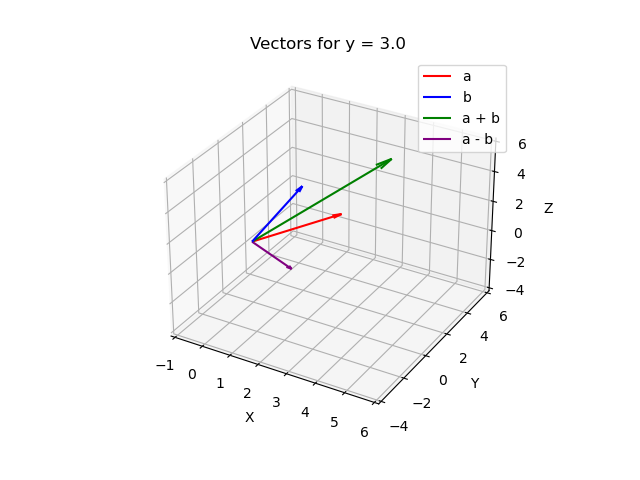
\includegraphics[width=1\columnwidth]{figs/fig1.png}
             \caption{Plot of vectors when y=3 }
             \label{fig:fig1}
         \end{figure}
         \begin{figure}
             \centering
             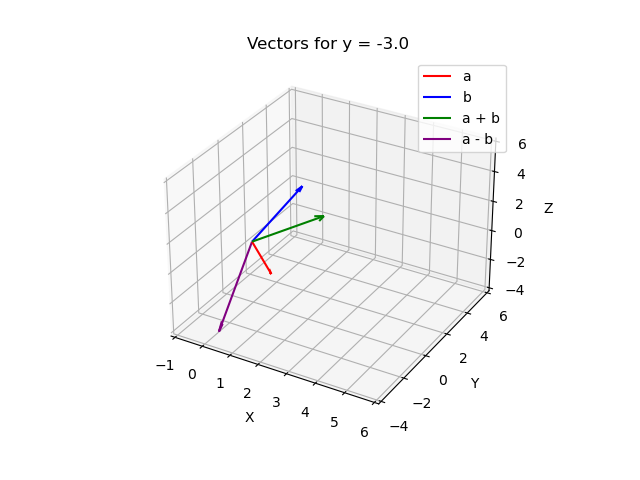
\includegraphics[width=1\linewidth]{figs/fig2.png}
             \caption{Plot of the vectors when y=-3}
             \label{fig:placeholder}
         \end{figure}
         
\end{document}
